% !TeX spellcheck = fr_FR
\chapter{Chapitre 0 : Base Technique}

Ce chapitre a pour but d'introduire et expliquer brièvement les différents aspects techniques clés de ce projet de semestre.

\section{FPGA}


\section{Fonction de hachage}

Une fonction de hachage\footnote{TO DO} est une fonction qui va prendre en entrée une donnée a taille variable et va ressortir une donnée de taille fixe. Une des particularités d'une fonction de hachage est qu'il n'est pas possible par calcul de retrouver la donnée qui a été donnée en entrée à partir d'un hash. En effet, la moindre différence sur la donnée en entrée va nous donner un hash en sortie qui n'a rien à voir. Cette particularité va permettre de sécuriser le stockage de mot de passe car même compromis, il ne devrait pas être possible de retrouver aisément les mots de passes.

\begin{figure}[tbph!]
	\centering
	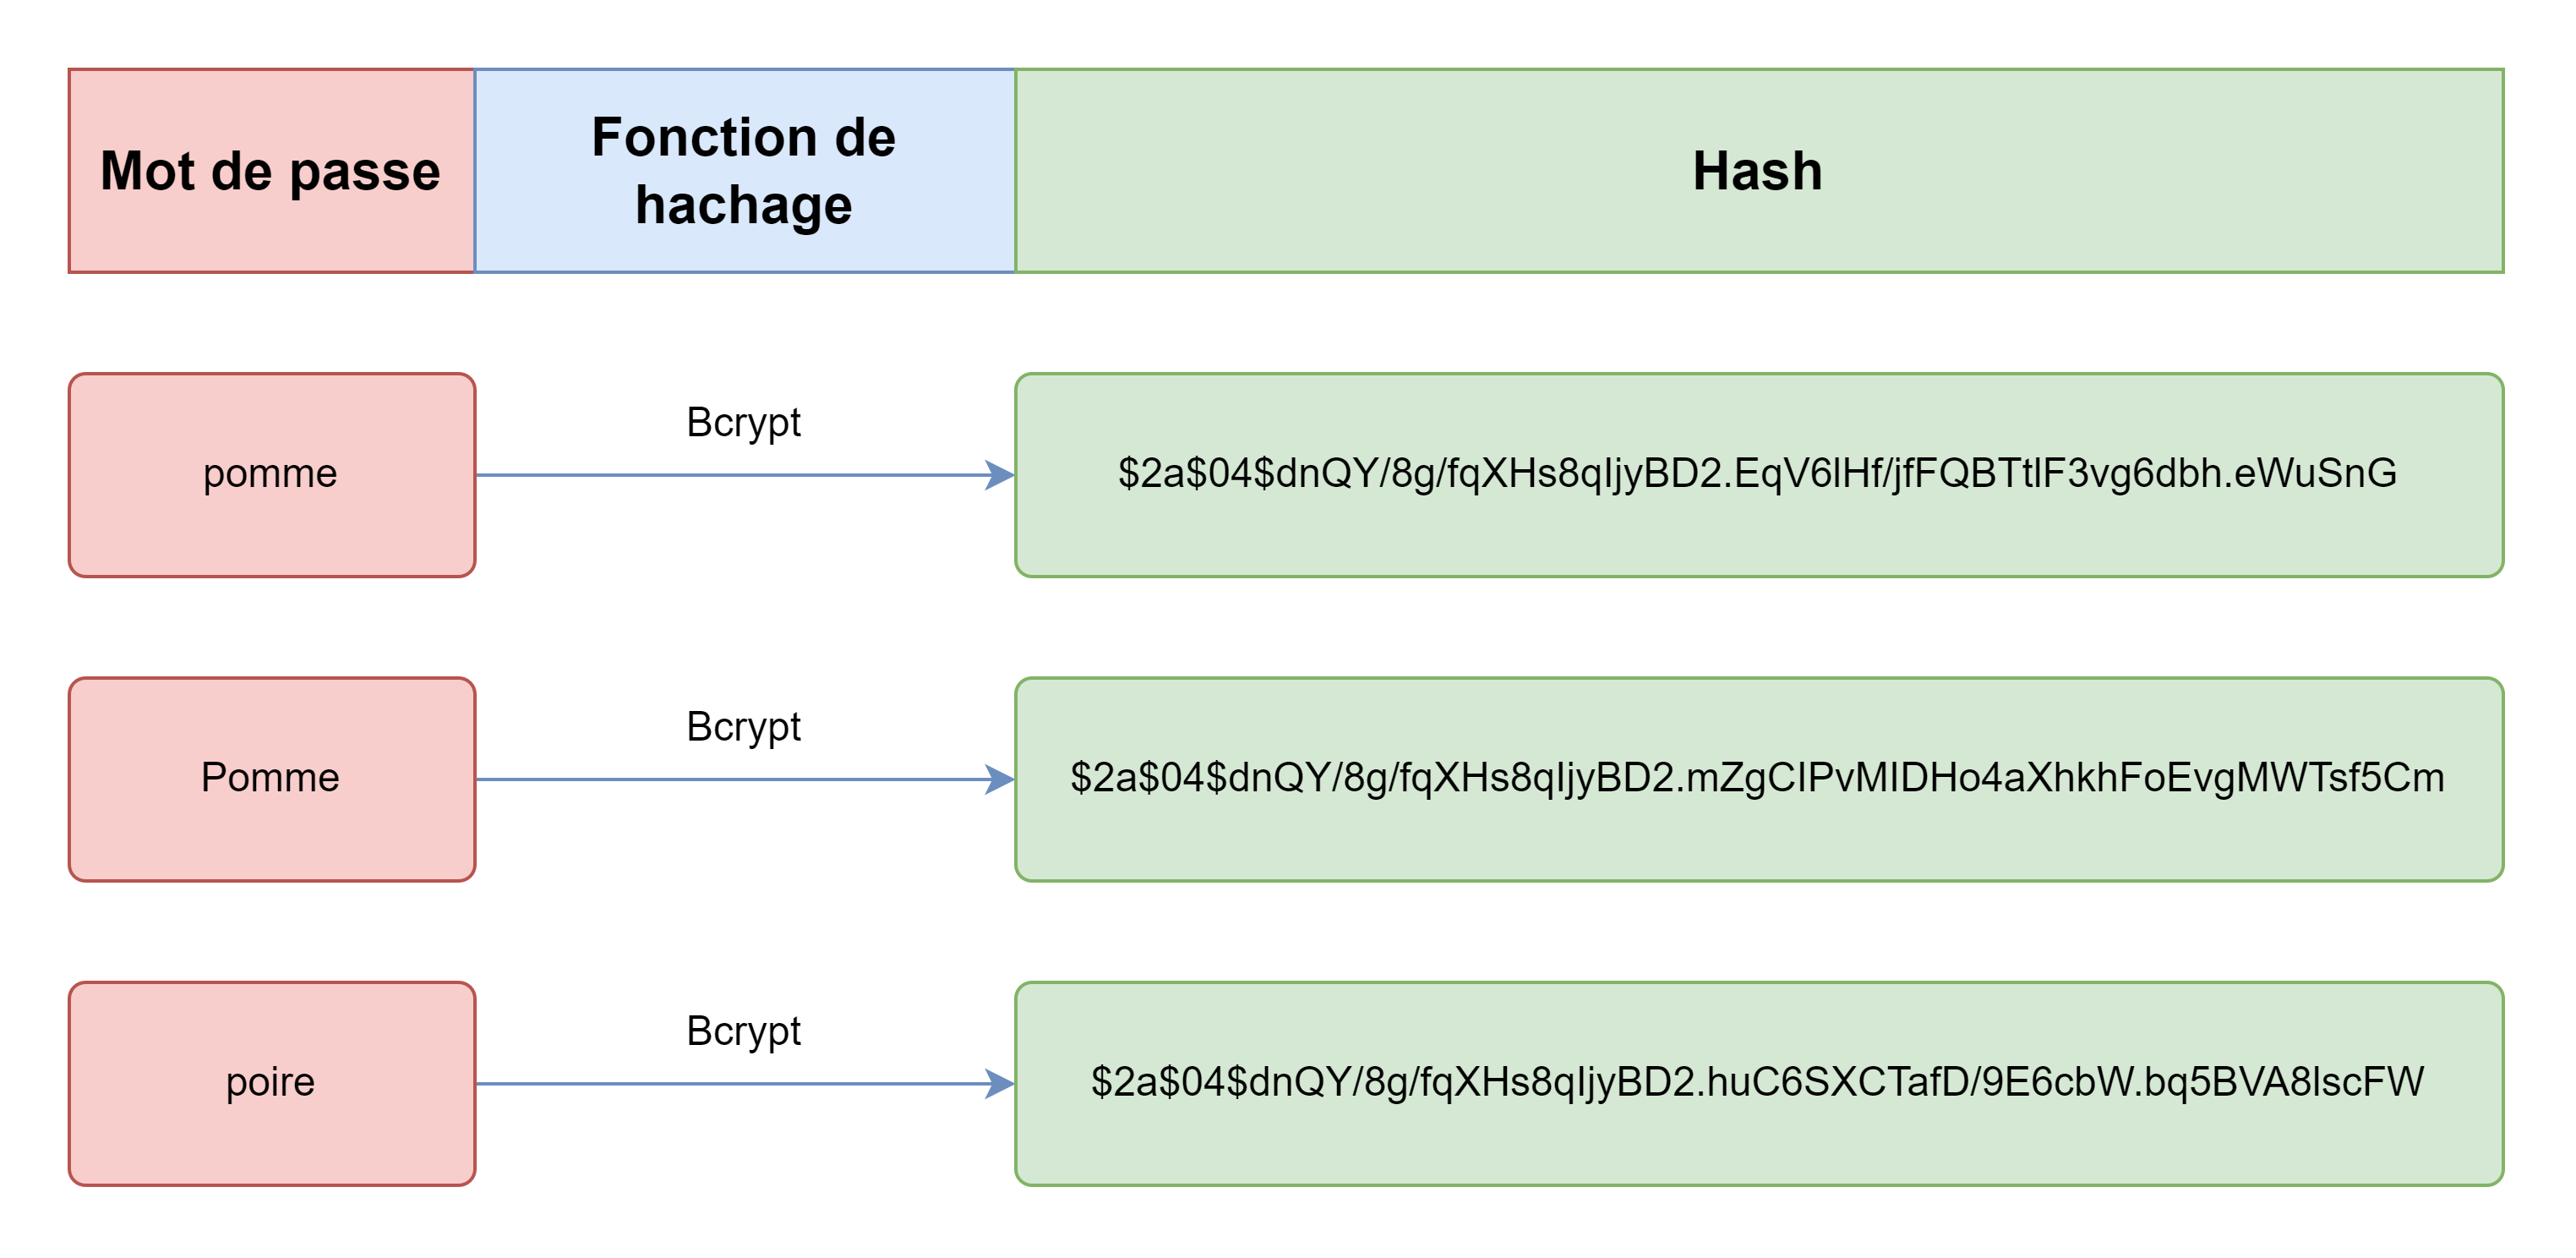
\includegraphics[width=0.7\linewidth]{hash_function}
	\caption[Fonction de hachage]{Fonction de hachage. Source : réalisé par Kandiah Abivarman}
	\label{fig:fonction_hachage}
\end{figure}


\subsection{Salt}



\subsection{Attaque par bruteforce}

